\documentclass{article}
\usepackage[utf8]{inputenc}
\usepackage{graphicx}
\usepackage{float}
\usepackage{hyperref}
\usepackage{listings}
\usepackage{amsmath}
\usepackage{xcolor}

\lstdefinelanguage{java}
{morekeywords=[1]{public,private,protected,class,interface,implements,extends,this,null,super,return,static,new,if,else,switch,case,while,for,do,break,continue,final,synchronized,try,catch,true,false,enum,assert,throw,throws,abstract,import},
morekeywords=[2]{double,float,long,int,short,byte,char,boolean,void},
morekeywords=[3]{String,System,BufferedReader,FileReader,IOException,BufferedWriter,FileWriter,ArithmeticException,Exception,List,ArrayList,Collections,Integer,Hashtable,Map,Runtime,StringBuilder},
morekeywords=[4]
{@Override},
morestring=[b]{"},
morecomment=[l]{//},
morecomment=[s]{/*}{*/},}

\lstset{
    frame=single,
    language=Java,                 % the language of the code
    breaklines=true,
    postbreak=\raisebox{0ex}[0ex][0ex]{\ensuremath{\color{red}\hookrightarrow\space}},
    extendedchars=true,
    literate={à}{{\`a}}1 {è}{{\`e}}1 {ã}{{\~a}}1 {é}{{\'e}}1,
}
\lstset{basicstyle=\fontsize{7}{8}\selectfont\tt}
\lstset{keywordstyle=[1]\color[rgb]{0,0,1}\bfseries}
\lstset{keywordstyle=[2]\color[rgb]{0.6,0,0}\bfseries}
\lstset{keywordstyle=[3]\color[rgb]{0,0.6,0}\bfseries}
\lstset{identifierstyle=\color{black}}
\lstset{commentstyle=\color[rgb]{0,0.6,0.6}}
\lstset{stringstyle=\color[rgb]{0.44,0.47,1}}
\lstset{showstringspaces=false}
\lstset{showtabs=false}
\lstset{tabsize=3}
\lstset{extendedchars=true}
\lstset{breaklines=true}
\lstset{postbreak={}}
\lstset{breakautoindent=true}
\lstset{breakindent=0pt}
\lstset{xleftmargin=0.1cm}
\lstset{xrightmargin=1mm}
\lstset{frame=shadowbox,rulecolor=\color[gray]{.2},rulesepcolor=\color[gray]{.75},framesep=2pt,backgroundcolor=\color[rgb]{1,1,0.9}}
\lstset{captionpos=b}
\lstset{aboveskip=0.5cm,belowskip=0.5cm}
\lstset{numbers=left}
\lstset{numberstyle=\tiny}
\lstset{columns=fixed}
\lstset{escapechar=§}
\lstset{language=java}

\usepackage{geometry}
\geometry{a4paper, portrait, margin=0.99in}

\newcommand{\codelocation}[2]{
	Le code se trouve dans le projet \texttt{#1} dans la classe \texttt{#2}.
}
\newcommand{\code}[2]{
	\codelocation{#1}{#2}
	\lstinputlisting{#1/#2}
}

\title{LSINF1113 - Algorithmique numérique\\Exercices}
\author{Denis Mortier}
\date{Décembre 2016}

\begin{document}

\maketitle

Ce document reprends les réponses aux questions des exercices proposés pour chaque $lecture$. Malgré le soin apporté à sa réalisation, aucune garantie n'est apportée quant à l'exactitude des réponses et chacun est invité à aider à compléter ou corriger ce document pour le rendre meilleur. Le code \LaTeX de ce document est disponible sur GitHub\footnote{\url{https://github.com/Zibeline/LSINF1113-Exercices/}}.

Les projets Java liés se trouvent dans le même repo que ce fichier. Pour toutes les petites classes indépendantes, elles ont toutes été rassemblées dans le projet \texttt{littleclasses}. A nouveau, aucune garantie n'est apportée sur le fait que le code soit correct, encore moins sur le fait qu'il soit optimal. Ici aussi chacun peut aider à les améliorer.

\section{Introduction and number representation}
\subsection{Question 1}

\begin{equation}
	\begin{aligned}
		RE &= |\frac{b-a}{b}|\\
		0.1 &= \frac{1}{2^5} + \frac{1}{2^6} + \frac{1}{2^8} + RE \\
		&= 0.1015625
	1\end{aligned}
\end{equation}

L'erreur est donc de $|\frac{0.1015625 - 0.1}{0.1}| = 0.015625$ soit une erreur de moins de 5 \%.

Rien que pour représenter la partie décimale, il faut donc 8 bits. Cela ne tiens pas compte ni du bit pour le signe ni des bits pour représenter la partie entière.

\subsection{Question 2}

\begin{equation}
	\begin{aligned}
		x &= [\underline{x}, \overline{x}]\\
		y &= [\underline{y}, \overline{y}]
	\end{aligned}
\end{equation}

On peut donc calculer la somme et le produit de $x$ et $y$ de cette manière :

\begin{equation}
	\begin{aligned}
		x + y &= [\underline{x} + \underline{y}, \overline{x} + \overline{y}]\\
		x \cdot y &= [\underline{x} \cdot \underline{y}, \overline{x} \cdot \overline{y}]
	\end{aligned}
\end{equation}

\subsection{Question 3}

\subsubsection{Point 1}

\paragraph{Très petit x}
Si $x_i \ll 0$, alors $e^x$ va devenir très petit. En effet, $e^{x} = \frac{1}{e^{|x|}}$ (pour $x$ négatif). $e^{|x|}$ sera donc grand et du coup $\frac{1}{e^{|x|}}$ sera très petit. On peut même dire que si $x$ est fortement négatif, $e^x$ tend vers 0. On obtiens alors $log(0+0+...+0) = log(0)$, ce qui est impossible. On aura donc une erreur lors de l'exécution de $log(0)$.

\paragraph{Très grand x}
Si $x_i \gg 0$, alors $e^x$ va devenir très grand, et on va très rapidement etteindra la capacité maximale et provoquer un $overflow$. On aura donc également une erreur, mais cette erreur aura lieu cette fois-ci dès le calcul de $e^x$.

\subsubsection{Point 2}

On peut remplacer chaque $x_i$ par $x_i-a+a$, où $a = max|\text{Valeur }x_i|$ :

\begin{equation}
	\begin{aligned}
		log(e^{a+x_i-a}+...+e^{a+x_i-a}) &= log (e^a(e^{x_i-a}+...+e^{x_i-a})\\
		&= log (e^a)+log(\sum e^{x_i-a})\\
		&= a+log(\sum e^{x_i-a})\\
	\end{aligned}
\end{equation}

\subsection{Question 4}

La méthode main contient deux variables, \texttt{start} et \texttt{end} qui déterminent les bornes où évaluer la fonction. La variable \texttt{pointsToCalculate} détermine le nombre de points à calculer. Les points seront répartis de manière uniforme entre \texttt{start} et \texttt{end}.

\code{littleclasses}{expo.java}

Et voici le graphique généré via gnuplot\footnote{\url{http://www.gnuplot.info}} avec comme paramètre \texttt{pointsToCalculate} à 100 :

\begin{figure}[H]
	\caption{\label{ex} Plot avec 100 points de calcul}
	\centering
	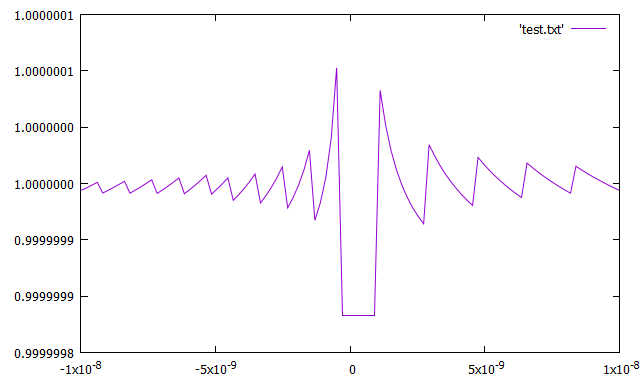
\includegraphics[scale = 0.61]{Figures/1_plot.png}
\end{figure}


\section{Matrix representation}
Tous les codes de cette leçon sont dans le projet \texttt{matrices}. En plus des codes demandés, plusieurs choses ont été imlémentées. D'une part une interface \texttt{Matrix} qui représente une matrice générique et une classe \texttt{Utilities} qui implémente plusieurs opérations sur les matrices (addition, affichage, ...).

\begin{figure}[H]
	\caption{\label{struc} Diagramme de la structure du projet "matrices"}
	\centering
	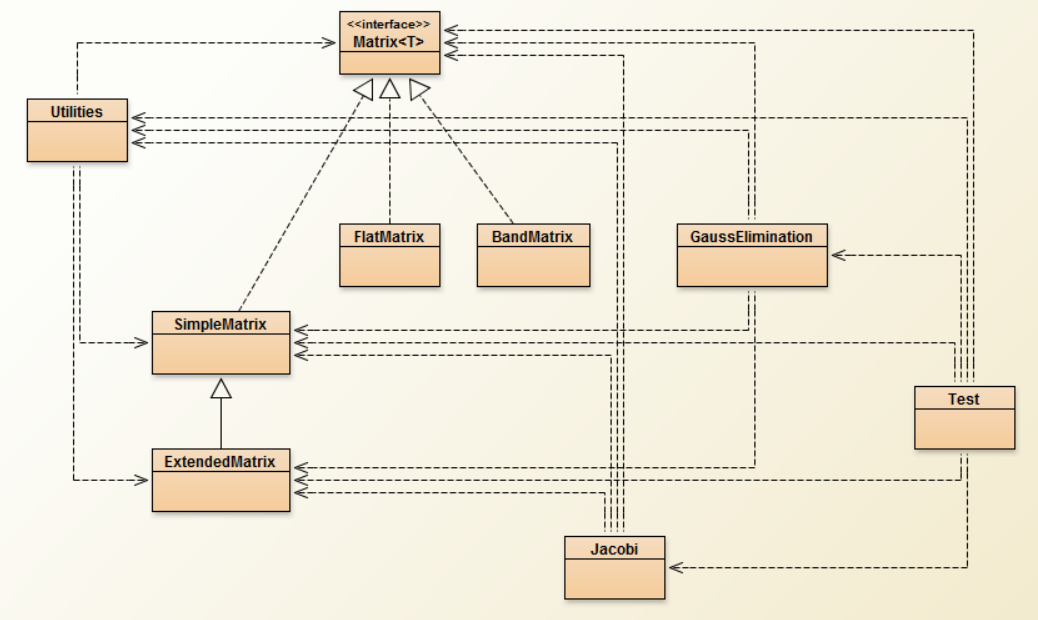
\includegraphics[scale = 0.6]{Figures/2_structure.png}
\end{figure}

Tous ce code est expérimental et ne peut pas être utilisé tel quel dans un projet. En effet, ils risquent de générer des erreurs, par exemple parce qu'ils ne vérifient jamais si les données sont correctement formatées. Le but est avant tout de se concentrer sur les algos et leur fonctionnement.

\subsection{Question 1}
\code{matrices}{FlatMatrix.java}

\subsection{Question 2}

// TO DO

\subsection{Question 3}

\subsubsection{Java representation of a band matrix}
\code{matrices}{BandMatrix.java}

\subsubsection{Multiplication by a band matrix}
\codelocation{matrices}{Utilities.java}
\begin{lstlisting}
public static Matrix multiplyByBand(Matrix base, Matrix band) {
    SimpleMatrix ret = new SimpleMatrix(base.getHeight(), base.getWidth());
    for (int i = 0; i < base.getHeight(); i++) {
        for (int j = 0; j < base.getWidth(); j++) {
            double pos = (double) base.get(i, j-1)* (double) band.get(j-1, j) + (double) base.get(i, j)*(double) band.get(j, j);
            ret.set(pos, i, j);
        }
    }
    return ret;
}
\end{lstlisting}

\section{Linear systems}
Les codes les codes de cette leçon sont également dans le projet "matrices". Dans la classe $Test.java$ se trouvent deux méthodes $\texttt{test\_gauss}$ et $\texttt{test\_jacobi}$ qui contiennent des matrices de test pour tester les deux méthodes.

\subsection{Question 1}
\code{matrices}{GaussElimination.java}

\subsection{Question 2}
\code{matrices}{Jacobi.java}

\section{Linear regression}
\subsection{Question 1}

\begin{equation}
	\begin{aligned}
		X^TXA &= X^TY\\
		\begin{pmatrix}
			1 & 1 & 1 & 1 & 1 & 1\\
			95 & 85 & 80 & 70 & 60 & 70
		\end{pmatrix}
		\cdot
		\begin{pmatrix}
			1 & 95 \\
			1 & 85 \\
			1 & 80 \\
			1 & 70 \\
			1 & 60 \\
			1 & 70 
		\end{pmatrix}
		\cdot
		\begin{pmatrix}
			a_1\\
			a_2
		\end{pmatrix}
		&=
		\begin{pmatrix}
			1 & 1 & 1 & 1 & 1 & 1\\
			95 & 85 & 80 & 70 & 60 & 70
		\end{pmatrix}
		\cdot
		\begin{pmatrix}
			85\\
			95\\
			70\\
			65\\
			70\\
			80
		\end{pmatrix}\\
		\begin{pmatrix}
			6 & 460\\
			460 & 36050
		\end{pmatrix}
		\cdot
		\begin{pmatrix}
			a_1\\
			a_2
		\end{pmatrix}
		&=
		\begin{pmatrix}
			465\\
			36100
		\end{pmatrix}\\
		\begin{pmatrix}
			1 & 36050/460\\
			6 & 460
		\end{pmatrix}
		\cdot
		\begin{pmatrix}
			a_1\\
			a_2
		\end{pmatrix}
		&=
		\begin{pmatrix}
			36100/460\\
			465
		\end{pmatrix}\\
		\begin{pmatrix}
			1 & 36050/460\\
			0 & 460 - 6 \cdot \frac{36050}{460}
		\end{pmatrix}
		\cdot
		\begin{pmatrix}
			a_1\\
			a_2
		\end{pmatrix}
		&=
		\begin{pmatrix}
			36100/460\\
			465-6 \cdot \frac{36100}{460}
		\end{pmatrix}\\
		\begin{pmatrix}
			1 & 36050/460\\
			0 & 1
		\end{pmatrix}
		\cdot
		\begin{pmatrix}
			a_1\\
			a_2
		\end{pmatrix}
		&=
		\begin{pmatrix}
			36100/460\\
			\frac{465-6 \cdot \frac{36100}{460}}{460 - 6 \cdot \frac{36050}{460}}
		\end{pmatrix}\\
		\begin{pmatrix}
			1 & 36050/460\\
			0 & 1
		\end{pmatrix}
		\cdot
		\begin{pmatrix}
			a_1\\
			a_2
		\end{pmatrix}
		&=
		\begin{pmatrix}
			36100/460\\
			\frac{27}{47}
		\end{pmatrix}\\
		\begin{pmatrix}
			1 & 0\\
			0 & 1
		\end{pmatrix}
		\cdot
		\begin{pmatrix}
			a_1\\
			a_2
		\end{pmatrix}
		&=
		\begin{pmatrix}
			36100/460-\frac{27}{47} \cdot 36050/460\\
			\frac{27}{47}
		\end{pmatrix}
	\end{aligned}
\end{equation}

\begin{equation}
	\begin{aligned}    
		a_1 &= 33,457\\
		a_2 &= 0.5745
	\end{aligned}
\end{equation}

\subsection{Question 2}

\subsubsection{Explicit normal equation for the model $y = a_1 + a_2x$}

\begin{equation}
	\begin{aligned}
		\begin{pmatrix}
			m & \displaystyle\sum_{i=1}^{m} x_i\\
			\displaystyle\sum_{i=1}^{m} x_i & \displaystyle\sum_{i=1}^{m} x_i^2
		\end{pmatrix}
		\cdot
		\begin{pmatrix}
			a_1\\
			a_2
		\end{pmatrix}=
		\begin{pmatrix}
			\displaystyle\sum_{i=1}^{m} y_i\\
			\displaystyle\sum_{i=1}^{m} x_iy_i
		\end{pmatrix}
	\end{aligned}
\end{equation}

\subsubsection{Explicit normal equation for the model $y = a_1 + a_2x + a_3x^2$}

\begin{equation}
	\begin{aligned}
		\begin{pmatrix}
			m & \displaystyle\sum_{i=1}^{m} x_i & \displaystyle\sum_{i=1}^{m} x_i^2\\
			\displaystyle\sum_{i=1}^{m} x_i & \displaystyle\sum_{i=1}^{m} x_i^2 & \displaystyle\sum_{i=1}^{m} x_i^3\\
			\displaystyle\sum_{i=1}^{m} x_i^2 & \displaystyle\sum_{i=1}^{m} x_i^3 & \displaystyle\sum_{i=1}^{m} x_i^4\\
		\end{pmatrix}
		\cdot
		\begin{pmatrix}
			a_1\\
			a_2\\
			a_3
		\end{pmatrix}=
		\begin{pmatrix}
			\displaystyle\sum_{i=1}^{m} y_i\\
			\displaystyle\sum_{i=1}^{m} x_iy_i\\
			\displaystyle\sum_{i=1}^{m} x_i^2y_i
		\end{pmatrix}
	\end{aligned}
\end{equation}


\subsection{Question 3}

\subsubsection{Point 1}

\begin{equation}
	\begin{aligned}
		A &= 
		\begin{pmatrix}
			25 & 15 & -5\\
			15 & 18 & 0\\
			-5 & 0 & 11\\
		\end{pmatrix};
		L_A = 
		\begin{pmatrix}
			5 & 0 & 0\\
			3 & 3 & 0\\
			-1 & 1 & 3\\
		\end{pmatrix}\\
		B &= 
		\begin{pmatrix}
			4 & 12 & -16\\
			12 & 37 & -43\\
			-16 & -43 & 98
		\end{pmatrix};
		L_B =
		\begin{pmatrix}
			2 & 0 & 0\\
			6 & 1 & 0\\
			-8 & 5 & 3
		\end{pmatrix}
	\end{aligned}
\end{equation}

Le fonctionnement de l'algorithme est développé en détail sur Wikipédia \footnote{https://fr.wikipedia.org/wiki/Factorisation\_de\_Cholesky\#Algorithme}.

\code{matrices}{CholeskyFactorization.java}

\subsubsection{Point 2}

\begin{equation}
	\begin{aligned}
		A=\begin{pmatrix}
		a & b\\
		c & d
		\end{pmatrix}
	\end{aligned}
\end{equation}

La matrice $A$ est positive définie si $Z^TAZ > 0$, pour un $Z$ non nul quelconque dans $R^n$.

\begin{equation}
	\begin{aligned}
		\begin{pmatrix}
		z_1 & z_2
		\end{pmatrix}\cdot
		\begin{pmatrix}
		a & b\\
		c & d
		\end{pmatrix}\cdot
		\begin{pmatrix}
		z_1\\
		z_2
		\end{pmatrix} &> 0\\
		\begin{pmatrix}
		z_1\cdot a + z_2\cdot c & z_1\cdot b + z_2\cdot d
		\end{pmatrix}\cdot
		\begin{pmatrix}
		z_1\\
		z_2
		\end{pmatrix} &> 0\\
		z_1^2\cdot a + z_1\cot z_2\cdot c + z_1 \cdot z_2 \cdot b + z_2^2\cdot d &> 0
	\end{aligned}
\end{equation}

Vu que $Z \neq 0$, $z_1$ et $z_2$ ne peuvent pas être nuls en même temps.

\begin{equation}
	\begin{aligned}
		z_1=0; z_2 \neq 0 \rightarrow &\quad z_2^2d>0\\
		&\quad d>0\\
		z_1\neq 0; z_2 = 0 \rightarrow &\quad z_1^2a>0\\
		&\quad a>0\\
	\end{aligned}
\end{equation}

$z_1^2$ et $z_2^2$ étant forcément plus grands que $0$ car ils sont non nuls et au carré, donc forcément positif.

\subsubsection{Point 3}

// TO DO

\section{Matrix norm and condition}
\subsection{Question 1}

Nous allons donc vérifier les 3 propriétés :

\begin{enumerate}
    \item $||A + B|| \leq ||A|| + ||B||$
    \item $||A \cdot W|| \leq ||A|| \cdot ||W||$
    \item $||A \cdot B|| \leq ||A|| \cdot ||B||$
\end{enumerate}

\paragraph{1e propriété}

\begin{equation}
	\begin{aligned}
		||A + B|| &= max_{||V||=1}||(A + B)V||\\
		&= max_{||V||=1}||AV + BV||\\
		&= max_{||V||=1}||AV|| + max_{||V||=1}||BV||\\
	\end{aligned}
\end{equation}

On peut passer de la deuxième à la troisième ligne car quand on multiplie une matrice par un vecteur on obtient un vecteur, et on peut donc appliquer les propriétés des vecteurs.

D'autre part on a que :

\begin{equation}
	\begin{aligned}
		||A|| + ||B|| &= max_{||V||=1}||AV|| + max_{||V||=1}||AV||
	\end{aligned}
\end{equation}

\paragraph{2e propriété}

Pour le cas ou $W = 0$, on sait que multiplier une matrice par un vecteur nul donne un vecteur nul, et que la norme d'un vecteur nul est nul.

\begin{equation}
	\begin{aligned}
		||A \cdot W|| &= ||A \cdot 0||\\
		&= ||0||\\
		&= 0
	\end{aligned}
\end{equation}


\begin{equation}
	\begin{aligned}
		||A|| \cdot ||W|| &= ||A|| \cdot ||0||\\
		&= ||A|| \cdot ||0||\\
		&= 0
	\end{aligned}
\end{equation}

Pour le cas ou $W \neq 0$ 

\paragraph{3e propriété}

// TO DO

\subsection{Question 2}

Trouvons juste un contre exemple.

\begin{equation}
	A = 
	\begin{pmatrix}
		1 & 2\\
		3 & 4
	\end{pmatrix};\\
	B = 
	\begin{pmatrix}
		5 & 6\\
		7 & 8
	\end{pmatrix};\\
	C = A \cdot B = 
	\begin{pmatrix}
		19 & 22\\
		43 & 50
	\end{pmatrix}
\end{equation}

\begin{equation}
	\begin{aligned}
		||A \cdot B|| &= ||C|| = max_{i,j}|c_{i,j}| = 50\\
		||A|| \cdot ||B|| &= max_{i,j}|a_{i,j}| \cdot max_{i,j}|b_{i,j}| = 4 \cdot 8 = 32\\
	\end{aligned}
\end{equation}

Pour que la norme soit sub-multiplicative il faut que $||A \cdot B|| \leq ||A|| \cdot ||B||$. Or 50 n'est pas plus petit ou égal à 32, donc cette norme ne peut être sub-multiplicative.

\subsection{Question 3}

Pour cette question toutes les matrices inverses ont été calculées via \href{http://matrixcalc.org/en/}{Matrixcalc.org}. Pour des matrices 2x2 on peut aisément le faire "à la main" avec la formule suivantes :

\begin{equation}
	\begin{aligned}
		A = 
		\begin{pmatrix}
			a & b\\
			c & d
		\end{pmatrix}; A^{-1} = 
		\begin{pmatrix}
			a & b\\
			c & d
		\end{pmatrix}^{(-1)} = 
		\frac{1}{ad-bc}
		\begin{pmatrix}
			d & -b\\
			-c & a
		\end{pmatrix}
	\end{aligned}
\end{equation}

La condition pour appliquer cette méthode étant que $ad - bc \neq 0$ (sinon on divise par zéro, et ça on ne peut pas faire).

\subsubsection{Point 1}

\begin{equation}
	\begin{aligned}
		Cond (A) &= ||A|| \cdot ||A^{-1}||\\
		||\cdot||_1 &= max_{1 \leq j \leq n} \sum_{i=1}^m|a_{ij}|\\
		\begin{pmatrix}
			2 & 3\\
			3 & 4
		\end{pmatrix}^{(-1)} = 
		\begin{pmatrix}
			-4 & 3\\
			3 & -2
		\end{pmatrix}\\
			||A|| &= 7\\
			||A||^{(-1)} &= 7\\
			Cond (A) &= 7 \cdot 7 = 49
	\end{aligned}
\end{equation}

\subsubsection{Point 2}

\begin{equation}
	\begin{aligned}
		\begin{pmatrix}
			2 & 2.2\\
			3 & 3.2
		\end{pmatrix}^{(-1)} = 
		\begin{pmatrix}
			-16 & 11\\
			15 & -10
		\end{pmatrix}\\
		||A|| &= 5.4\\
		||A||^{(-1)} &= 31\\
		Cond (A) &= ||A|| \cdot ||A^{-1}||\\
		&= 5.4 \cdot 31 = 167.4
	\end{aligned}
\end{equation}

On ne peut rien dire sur le condition number sans avoir calculé $A^{-1}$.

\subsubsection{Point 3}

\begin{equation}
	\begin{aligned}X = 
		\begin{pmatrix}
			2 & 2.2\\
			3 & 3.2
		\end{pmatrix}; Y = 
		\begin{pmatrix}
			3\\
			4
		\end{pmatrix}
	\end{aligned}
\end{equation}

// TO DO

\section{Interpolation}
\subsection{Question 1}

\subsubsection{Vandermonde}

\begin{equation}
	\begin{aligned}
		\begin{pmatrix}
			1 & 12 & 144\\
			1 & 20 & 400\\
			1 & 24 & 576
		\end{pmatrix}
		\cdot
		\begin{pmatrix}
			a_1\\
			a_2\\
			a_3
		\end{pmatrix}=
		\begin{pmatrix}
			4\\
			16\\
			17
		\end{pmatrix}
	\end{aligned}
\end{equation}

On peut ensuite trouver les valeurs $a_1$, $a_2$ et $a_3$ en résolvant le système.

Ici, nous n'avons pas fait ce développement, nous avons simplement entré la matrice dans la méthode de résolution par Gauss-Jordan implémentée dans la première question de la leçon 3.

Nous obtenons ainsi :

\begin{equation}
	\begin{aligned}
		a_1 &= -39\\
		a_2 &= 4.833\\
		a_3 &= -0.104
	\end{aligned}
\end{equation}

\subsubsection{Lagrange}

\begin{equation}
	f(x) = (y^{(1)} \cdot \Phi_1(x)) + (y^{(2)} \cdot \Phi_2(x)) + (y^{(3)} \cdot \Phi_3(x))
\end{equation}

\begin{equation}
	\begin{aligned}
		\Phi_1(x) &= \frac{(x-x^{(2)})(x-x^{(3)})}{(x^{(1)}-x^{(2)})(x^{(1)}-x^{(3)})} = \frac{(x-20)(x-24)}{96} = \frac{x^2}{96} - \frac{11}{24}x+5\\
		\Phi_1(x) &= \frac{(x-x^{(1)})(x-x^{(3)})}{(x^{(2)}-x^{(1)})(x^{(2)}-x^{(3)})} = \frac{(x-12)(x-24)}{-32} = \frac{-3x^2}{96} + \frac{27}{24}x - 9\\
		\Phi_1(x) &= \frac{(x-x^{(1)})(x-x^{(2)})}{(x^{(3)}-x^{(1)})(x^{(3)}-x^{(2)})} = \frac{(x-12)(x-20)}{48} = \frac{2x^2}{96} - \frac{16}{24}x + 5
	\end{aligned}
\end{equation}


\begin{equation}
	\begin{aligned}
		f(x) = \frac{-5}{48}x^2 + \frac{29}{6}x-144
	\end{aligned}
\end{equation}

\subsubsection{Newton}

\begin{equation}
	\begin{aligned}
		\Psi_1(x) &= 1\\
		\Psi_2(x) &= \Psi_1(x) \cdot (x-12)\\
		\Psi_3(x) &= \Psi_2(x) \cdot (x-20) = (x-12)(x-20)\\
	\end{aligned}
\end{equation}

\begin{equation}
	\begin{pmatrix}
		1 & 0 & 0\\
		1 & 8 & 0\\
		1 & 12 & 48
	\end{pmatrix}\cdot
	\begin{pmatrix}
		c_1\\
		c_2\\
		c_3
	\end{pmatrix}=
	\begin{pmatrix}
		4\\
		16\\
		17
	\end{pmatrix}
\end{equation}

A l'aide de notre méthode Java pour Gauss-Jordan, nous obtenons que 

\begin{equation}
	\begin{aligned}
		c_1 &= 4\\
		c_2 &= 1.5\\
		c_3 &= -0.104
	\end{aligned}
\end{equation}

Nous pouvons alors définir $f(x)$ :

\begin{equation}
	f(x) = 4 + 1.5(x-12) - 0.104(x-12)(x-20)
\end{equation}


\begin{figure}[H]
\caption{\label{3pts} Interpolation avec 3 points}
\centering
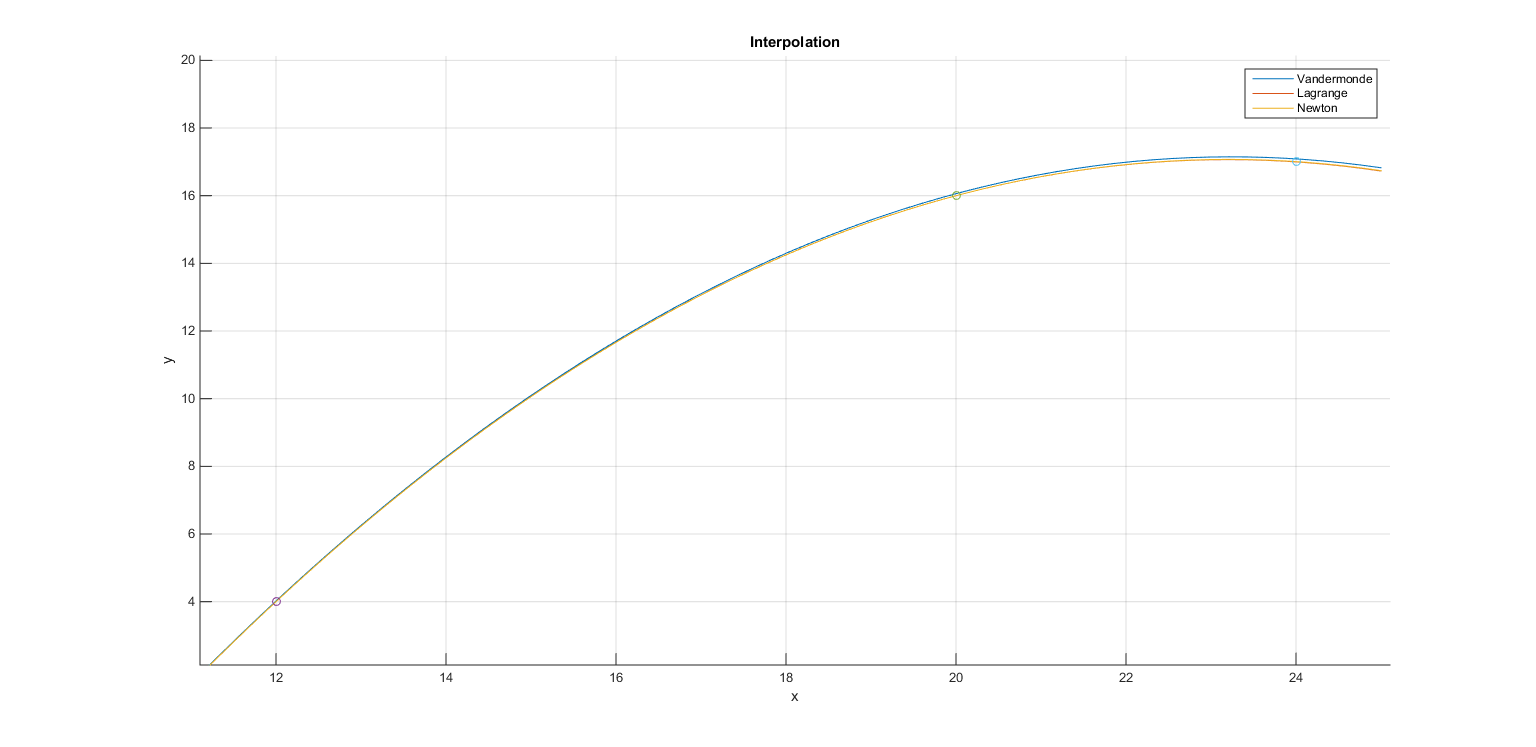
\includegraphics[scale = 0.4]{Figures/6_interpolation.png}
\end{figure}

\subsubsection{Vandermonde avec une mesure en plus}

\begin{equation}
	\begin{aligned}
		\begin{pmatrix}
			1 & 12 & 144 & 1728\\
			1 & 20 & 400 & 8000\\
			1 & 24 & 576 & 13824\\
			1 & 16 & 256 & 4096
		\end{pmatrix}
		\cdot
		\begin{pmatrix}
			a_1\\
			a_2\\
			a_3\\
			a_4
		\end{pmatrix}
		=
		\begin{pmatrix}
			4\\
			16\\
			17\\
			13
		\end{pmatrix}
	\end{aligned}
\end{equation}

On peut ensuite trouver les valeurs $a_1$, $a_2$, $a_3$ et $a_4$ en résolvant le système. Nous obtenons ainsi :

\begin{equation}
	\begin{aligned}
		a_1 &= -99\\
		a_2 &= 46/3\\
		a_3 &= -11/16\\
		a_4 &= 1/96
	\end{aligned}
\end{equation}

\subsubsection{Newton avec une mesure en plus}

\begin{equation}
	\begin{aligned}
		f(x) &= 4 + 1.5(x-12) - 0.104(x-12)(x-20) + c_4(x-12)(x-20)(x-24)\\
		f(16) &= 13\\
		13 &= 10 + \frac{80}{48}+128c_4\\
		c_4 &= \frac{3-80/48}{128} = \frac{1}{96}
	\end{aligned}
\end{equation}

\begin{figure}[H]
	\centering
	\caption{\label{4pts} Interpolation avec 4 points}
	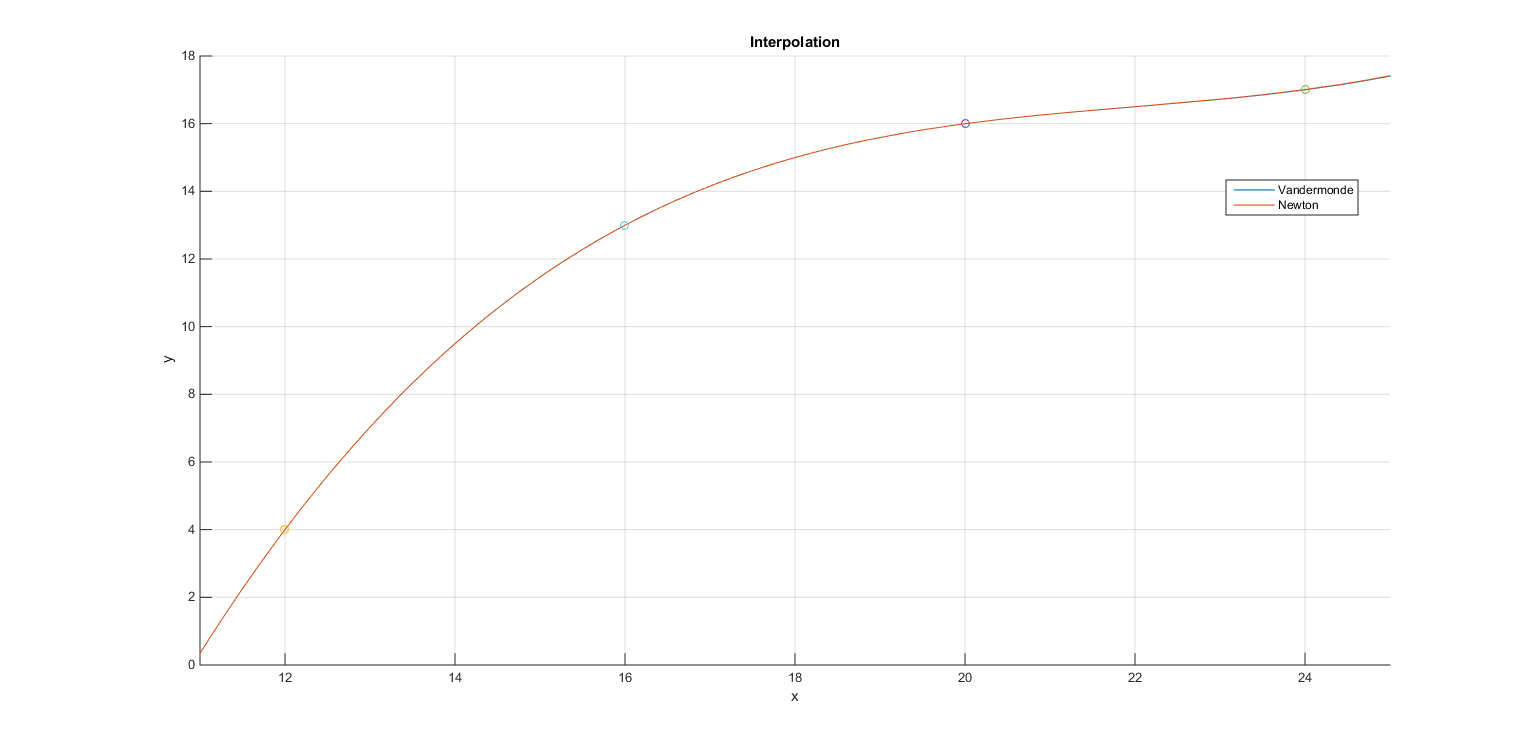
\includegraphics[scale = 0.4]{Figures/6_interpolation_2.png}
\end{figure}

\begin{figure}[H]
	\centering
	\caption{\label{3ou4} Interpolation via Newton avec 3 ou 4 points}
	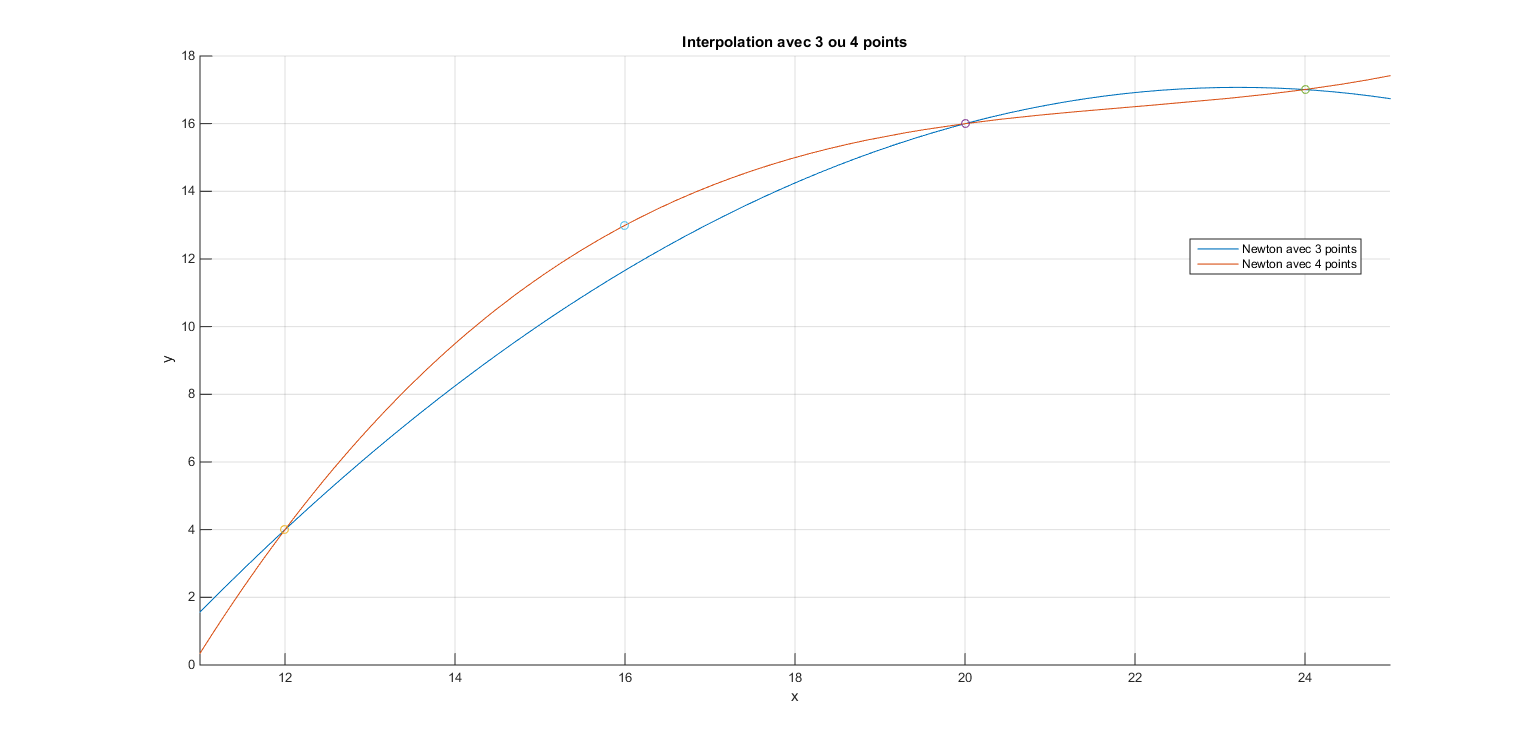
\includegraphics[scale = 0.4]{Figures/6_interpolation_3ou4.png}
\end{figure}


\subsection{Question 2}

Tous les codes de cette question sont dans le projet \texttt{numalgoplotter} qui est basé sur les codes fournis sur moodle. 

\subsubsection{NumAlgoPlotter}
\code{numalgoplotter}{NumAlgoPlotter.java}

\subsubsection{VandermondePlotter}
\code{numalgoplotter}{VandermondePlotter.java}

\begin{figure}[H]
	\centering
	\caption{\label{vandermonde} VandermondePlotter}
	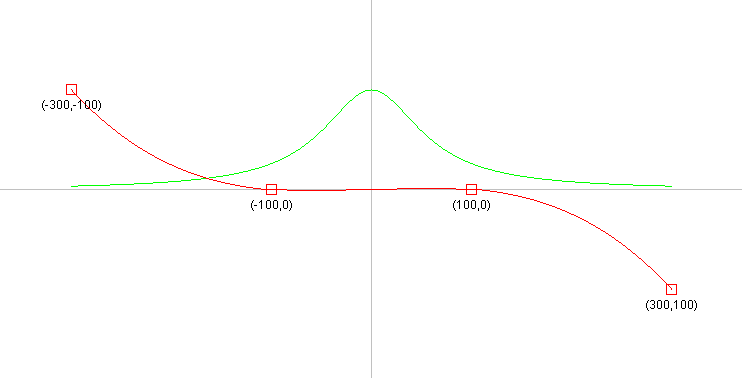
\includegraphics[scale = 0.4]{Figures/6_VandermondePlotter.png}
\end{figure}

\subsubsection{NewtonPlotter}
\code{numalgoplotter}{NewtonPlotter.java}

\begin{figure}[H]
	\centering
	\caption{\label{newton} NewtonPlotter}
	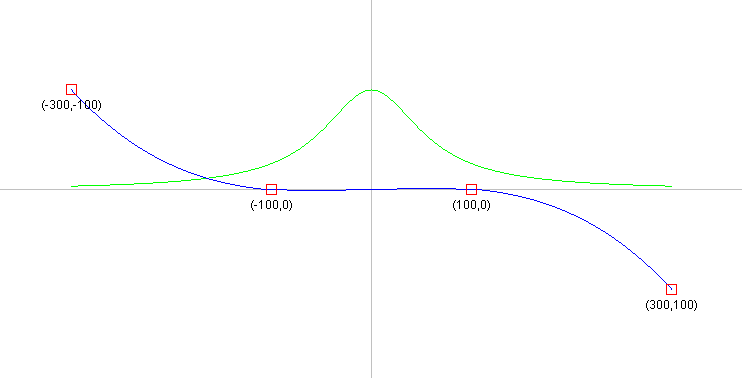
\includegraphics[scale = 0.4]{Figures/6_NewtonPlotter.png}
\end{figure}

\section{Splines}
Tous les codes de cette leçon sont comme pour la dernière leçon dans le projet \texttt{numalgoplotter} qui est basé sur les codes fournis sur moodle. 

\subsection{Question 1}
\code{numalgoplotter}{CubicSplinePlotter.java}

\begin{figure}[H]
	\centering
	\caption{\label{comparaison} Comparaison entre NewtonPlotter (en bleu) et CubicSplinePlotter (en noir)}
	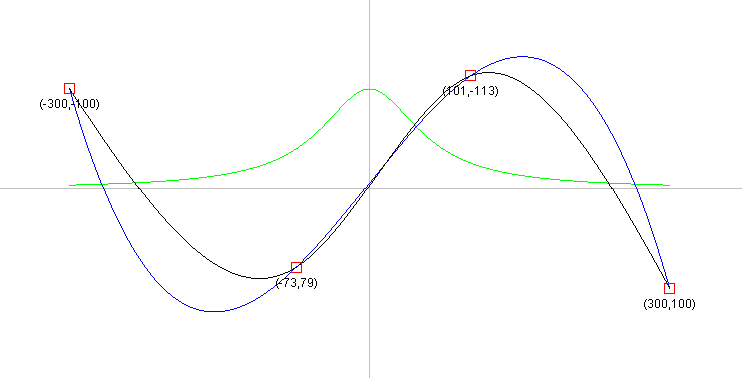
\includegraphics[scale = 0.4]{Figures/7_comparaisonNewtonCubic.png}
\end{figure}

\subsection{Question 2}

\code{numalgoplotter}{BSplinePlotter.java}

\begin{figure}[H]
	\caption{\label{7_zorro} Exemple de B-Spline}
	\centering
	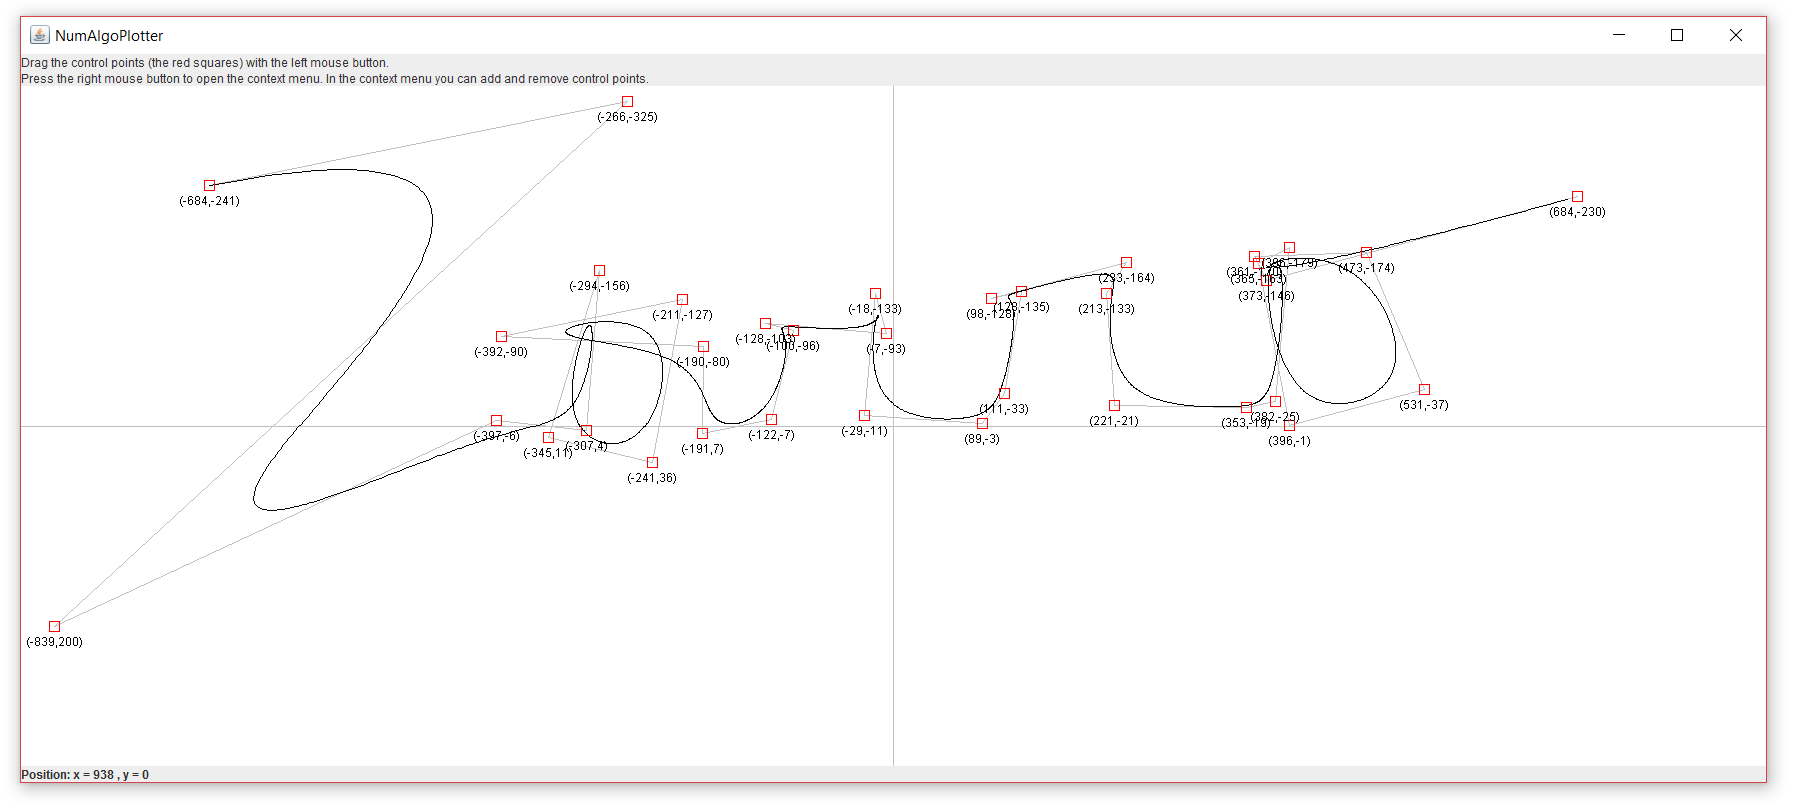
\includegraphics[scale = 0.3]{Figures/7_zorro.png}
\end{figure}

\subsection{Question 3}

// TO DO


\subsection{Question 4}

// TO DO

\section{Numerical integration}
\subsection{Question 1}

\subsubsection{Point 1}

Données :

\begin{equation}
	\begin{aligned}
		\int_a^b f(x) &\approx \sum_{i=1}^n f(x^{(i)}) \cdot h \cdot \int_1^n\frac{\prod_{j \neq i}(t-j)}{\prod_{j \neq i} (i - j)} dt\\
		n &= 3\\
		h &= \frac{b-a}{n-1} = \frac{b-a}{2}
	\end{aligned}
\end{equation}

Résolution :

\begin{equation}
	\begin{aligned}
		\int_a^b f(x) &\approx \sum_{i=1}^3 f(x^{(i)}) \cdot \frac{b-a}{2} \cdot \int_1^3\frac{\prod_{j \neq i}(t-j)}{\prod_{j \neq i} (i - j)} dt\\
		&= f(x^{(1)}) \cdot \frac{b-a}{2} \cdot \omega_1 + f(x^{(2)}) \cdot \frac{b-a}{2} \cdot \omega_2 + f(x^{(3)}) \cdot \frac{b-a}{2} \cdot \omega_3
	\end{aligned}
\end{equation}

On peut calculer les $\omega_i$ :

\begin{equation}
	\begin{aligned}
		\omega_1 &= \int_1^3 \frac{(t-2)(t-3)}{(1-2)(1-3)} dt\\
		&= \frac{1}{2} \int_1^3 t^2 - 5t + 6 dt\\
		&= \frac{1}{2} \left [\frac{t^3}{3} - \frac{5t^2}{2} + 6t \right ]_1^3\\
		&= \frac{1}{2}  \left [\frac{9}{2} - \frac{23}{6} \right ] = \frac{1}{3}\\
		\omega_2 &= \int_1^3 \frac{(t-3)(t-3)}{(2-1)(2-3)} dt\\
		&= -1 \int_1^3 t^2 - 4t + 3 dt\\
		&= -1  \left [\frac{t^3}{3} - 2t^2 + 3t \right ]_1^3\\
		&= -1  \left [ 0 - \frac{4}{3} \right ] = \frac{4}{3}\\
		\omega_3 &= \int_1^3 \frac{(t-1)(t-2)}{(3-1)(3-2)} dt\\
		&= \frac{1}{2} \int_1^3 t^2 - 3t + 2 dt\\
		&= \frac{1}{2}  \left [\frac{t^3}{3} - \frac{3t^2}{2} + 2t \right ]_1^3\\
		&= \frac{1}{2}  \left [ \frac{3}{2} - \frac{5}{6} \right ] = \frac{1}{3}\\
	\end{aligned}
\end{equation}

On peut alors remplacer les $\omega_i$ pour obtenir :

\begin{equation}
	\begin{aligned}
		\int_a^b f(x) &\approx f(a) \cdot \frac{b-a}{2} \cdot \frac{1}{3} + f(\frac{a+b}{2}) \cdot \frac{b-a}{2} \cdot \frac{4}{3} + f(b) \cdot \frac{b-a}{2} \cdot \frac{1}{3} \\
		&= \frac{b-a}{6} \left (f(a) + 4f(\frac{a+b}{2})+f(b) \right )
	\end{aligned}
\end{equation}

\subsubsection{Point 2}

// TO DO

\subsection{Question 2}

\subsubsection{Point 1}

// TO DO

\subsubsection{Point 2}

// TO DO

\subsubsection{Point 3}

// TO DO


\subsection{Question 3}

\subsubsection{Newton-Cotes with $n = 2$}

\begin{equation}
	\begin{aligned}
		\int_{-1}^2 e^x dx &\approx \sum_{i=1}^2 f(x^{(i)}) \cdot h \cdot \int_1^2\frac{\prod_{j \neq i}(t-j)}{\prod_{j \neq i} (i - j)} dt\\
		&= f(x^{(1)}) \cdot h \cdot \omega_1 + f(x^{(2)}) \cdot h \cdot \omega_2
	\end{aligned}
\end{equation}

On a que :

\begin{equation}
	\begin{aligned}
		n &= 2\\
		[a, b] &= [-1, 2]\\
		h &= \frac{b-a}{n-1} = 3
	\end{aligned}
\end{equation}

On peut calculer les $\omega_i$ :

\begin{equation}
	\begin{aligned}
		\omega_1 &= \int_1^2 \frac{(t-2)}{(1-2)} dt\\
		&= -\left [\frac{t^2}{2}-2t \right ]_1^2\\
		&= -\left [0 - (-3/2)\right] = \frac{-3}{2}\\
		\omega_2 &= \int_1^2 \frac{(t-1)}{(2-1)} dt\\
		&= \left [\frac{t^2}{2}-t \right ]_1^2\\
		&= \left [0 - (-1/2)\right] = \frac{1}{2}\\
	\end{aligned}
\end{equation}

On peut dès lors résoudre :

\begin{equation}
	\begin{aligned}
		\int_{-1}^2 e^x dx &\approx f(x^{(1)}) \cdot h \cdot \omega_1 + f(x^{(2)}) \cdot h \cdot \omega_2\\
		&= f(-1) \cdot 3 \cdot \frac{-3}{2} + f(2) \cdot 3 \cdot \frac{1}{2}\\
		&= e^{(-1)} \cdot 3 \cdot \frac{-3}{2} + e^2 \cdot 3 \cdot \frac{1}{2}\\
		&= 9.42812
	\end{aligned}
\end{equation}

L'erreur est donc de $9.42812 - 7.02118 = 2.40694$.

\subsubsection{Gauss-Legendre with $n = 2$}

Si on connais $\omega_i$ et $x^{(i)}$ pour $\int_{-1}^1$ on a que

\begin{equation}
	\begin{aligned}
		\int_a^b f(x) dx &= \frac{b-a}{2} \sum_{i=1}^n \omega_i f\left(\frac{b-a}{2}x^{(i)}+\frac{a+b}{2}\right)\\
		a &= -1\\
		b &= 2\\
		n &= 2
	\end{aligned}
\end{equation}

On va donc commencer par trouver $\omega_i$ et $x^{(i)}$.

\begin{equation}
	\begin{aligned}
		\sum_{j=1}^n \omega_j (x^{(i)})^{i-1} &= \frac{(b^i-a^i)}{i}\\
		i &= 1, ..., 2n\\
		\begin{cases}
		\omega_1+\omega_2 = 2\\
		\omega_1x^{(1)}+\omega_2 x^{(2)}= 0\\
		\omega_1x^{(1	)^2}+\omega_2 x^{(2)^2}= \frac{2}{3}\\
		\omega_1x^{(1)^3}+\omega_2 x^{(2)^3}= 0\\
		\end{cases}
		\omega_1 &= 1\\
		\omega_2 &= 1\\
		x^{(1)} &= -\frac{1}{\sqrt{3}}\\
		x^{(2)} &= \frac{1}{\sqrt{3}}\\
	\end{aligned}
\end{equation}

On peut alors appliquer la formule pour obtenir l'intégrale par Gauss-Legendre :

\begin{equation}
	\begin{aligned}
		\int_a^b f(x) dx &= \frac{b-a}{2} \sum_{i=1}^n \omega_i f\left(\frac{b-a}{2}x^{(i)}+\frac{a+b}{2}\right)\\
		&= \frac{2-(-1)}{2} \sum_{i=1}^2 \omega_i f\left(\frac{2-(-1)}{2}x^{(i)}+\frac{(-1)+2}{2}\right)\\
		&= \frac{3}{2} \left [\omega_1 f\left(\frac{3}{2}x^{(1)}+\frac{1}{2}\right) + \omega_2 f\left(\frac{3}{2}x^{(2)}+\frac{1}{2}\right)\right ]\\
		&= \frac{3}{2} \left [1 \cdot f\left(\frac{3}{2}\cdot\frac{-1}{\sqrt{3}}+\frac{1}{2}\right) + 1 \cdot f\left(\frac{3}{2}\cdot\frac{-1}{\sqrt{3}}+\frac{1}{2}\right)\right ]\\
		&= \frac{3}{2} \left [e^{\frac{-\sqrt{3}+1}{2}}+ e^{\frac{\sqrt{3}+1}{2}}\right ]\\
		&= \frac{3}{2} \left [e^{\frac{-\sqrt{3}+1}{2}}+ e^{\frac{\sqrt{3}+1}{2}}\right ]\\
		&= \frac{3}{2} \left[0.693485+3.919740\right]
		&=  6.91983
	\end{aligned}
\end{equation}

L'erreur est donc de $6.91983 -  7.02118 = -0.10135$, soit une erreur $\pm 23$ fois plus petite qu'avec la méthode de Newton-Cotes. La méthode de Gauss-Legendre donne donc le meilleur résultat.

\subsection{Question 4}

// TO DO


\subsection{Question 5}

// TO DO

\section{Ray tracing (part 1)}
Tous les codes de cette leçon sont dans le projet \texttt{raytracing} qui est basé sur les codes fournis sur moodle. 

\begin{figure}[H]
	\caption{\label{9_structure} Diagramme de la structure de raytracing}
	\centering
	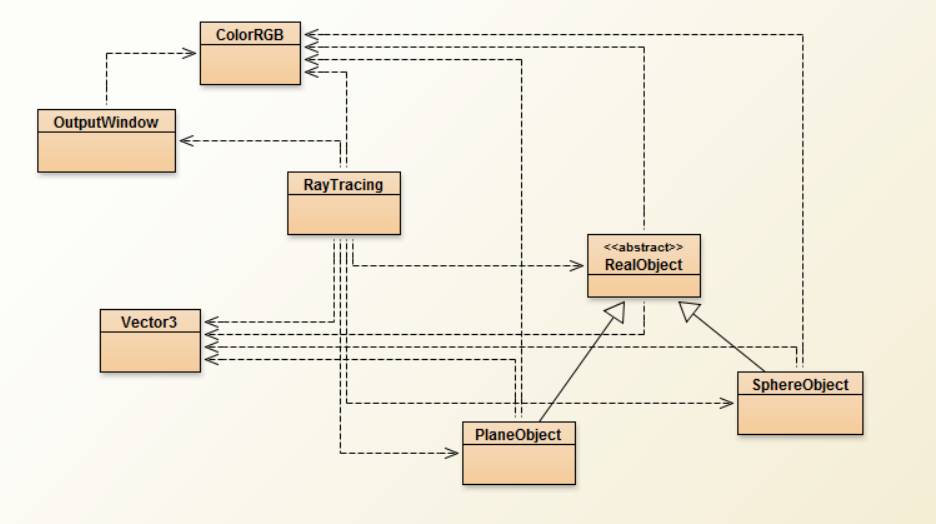
\includegraphics[scale = 0.4]{Figures/9_structure.png}
\end{figure}

\subsection{Question 1}

\subsubsection{Vector3}

Il y a dans cette classe quelques méthodes en plus de ce qui est demandé dans l'énoncé. Il s'agit de méthodes qui se sont révélées utiles par la suite lors de l'implémentation des autres méthodes.

\code{raytracing}{Vector3.java}

\subsubsection{ColorRGB}

Ici aussi, quelques méthodes complémentaires, qui seront utiles par la suite, ont été implémentées.

\code{raytracing}{ColorRGB.java}

\subsubsection{PlaneObject}
\code{raytracing}{PlaneObject.java}

\subsubsection{SphereObject}
\code{raytracing}{SphereObject.java}

\subsubsection{RayTracing}

La classe \texttt{RealObject} a du être adaptée pour que la couleur soit de type \texttt{ColorRGB} et non pas un \texttt{Vector3}.

\code{raytracing}{RayTracing.java}


\subsection{Question 2}

// TO DO

\subsection{Question 3}

Le code a directement été implementé. Il s'agit des deux denirères lignes de la méthode \texttt{traceRay} dans la classe \texttt{RayTracing}

\begin{lstlisting}
double distanceFactor = 120/Math.pow(tret, 2);
return ColorRGB.multiply(objectColor, distanceFactor);
\end{lstlisting}

\begin{figure}[H]
	\caption{\label{9_resultat} Résultat obtenu}
	\centering
	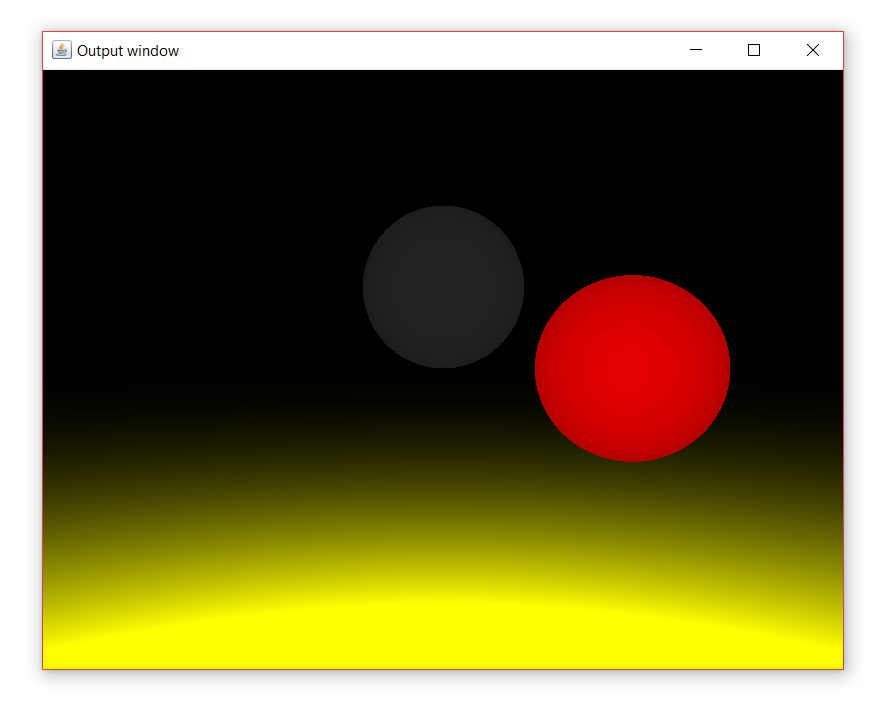
\includegraphics[scale = 0.4]{Figures/9_resultat.png}
\end{figure}

\section{Ray tracing (part 2)}
Tous les codes de cette leçon sont dans le projet \texttt{raytracing-extended} qui est basé sur le projet \texttt{raytracing} implémenté dans la leçon précédente.

\subsection{Question 1}

On va ici pour chaque étape décrire les modifications apportées au code, sans mettre les codes complets, pour les codes complets il suffira de se réferrer aux codes sources.

Dans les modifictions que nous allons apporter au code, nous allons devoir étendre la méthode \texttt{traceRay} de la classe \texttt{RayTracing}. Pour cela nous allons juste après le code qui permets de tester les collisions créer quatre variables qui nous servirons tout au long de ces modifications ;

\begin{lstlisting}
Vector3 ip = Vector3.add(rayPosition, Vector3.multiply(rayDirection, tret));
Vector3 normal = Vector3.normalize(hittedObject.getNormal(ip));
        
ColorRGB finalColor = new ColorRGB(0, 0, 0);
ColorRGB objectColor = hittedObject.getColor(ip);
\end{lstlisting}

\subsubsection{Diffuse reflection and ambient light}

On commence par créer une classe qui représente une lampe.

\code{raytracing-extended}{Lamp.java}

Une \texttt{LinkedList} de lampes est créée au début de \texttt{RayTracing}, ainsi qu'une couleur pour la lumière ambiante.

\begin{lstlisting}
LinkedList<Lamp> lamps=new LinkedList<>();
private ColorRGB ambientLight;
\end{lstlisting}

Dans le constructeur de RayTracing on peut alors ajouter des lampes et définir la couleur de la lumière ambiante.

\begin{lstlisting}
lamps.add(new Lamp(new Vector3(-10, 10, 10), new ColorRGB(0.9, 0.9, 0.9)));
lamps.add(new Lamp(new Vector3(5, 10, 10), new ColorRGB(0.5, 0.5, 0.5)));
ambientLight = new ColorRGB(0.3, 0.3, 0.3);
\end{lstlisting}

Les méthodes \texttt{getNormal} dans les classes représentant les objets avaient déjà été implémentées lors de la leçon précédente. Par exemple, voici la méthode pour la classe \texttt{SphereObject} :

\begin{lstlisting}
public Vector3 getNormal(Vector3 pointOnSurface) {
    Vector3 min = Vector3.subst(pointOnSurface, c);
    return new Vector3(min.x/radius, min.y/radius, min.z/radius);
}
\end{lstlisting}

On peut alors parcourir la liste des lampes pour calculer la couleur. Pour le fonctionnement du code, se réferrer à l'algorithme dans les slides. Pour finir, on ajoute également la lumière ambiante.

\begin{lstlisting}
// ***** Diffuse reflection and ambient light *****
for (int i = 0; i < lamps.size(); i++) {
    Lamp light = lamps.get(i);
    Vector3 dl = Vector3.normalize(Vector3.subst(light.pos, ip));
    double cosa = Vector3.dotProduct(normal, dl)/(Vector3.getLength(normal) * Vector3.getLength(dl));
    if (cosa>0) {
        finalColor.add(ColorRGB.multiply(light.color, objectColor, cosa));
    }
}
finalColor.add(ColorRGB.multiply(ambientLight, objectColor));
\end{lstlisting}

\begin{figure}[H]
	\caption{\label{10_1} Réflexion diffuse et lumière ambiante}
	\centering
	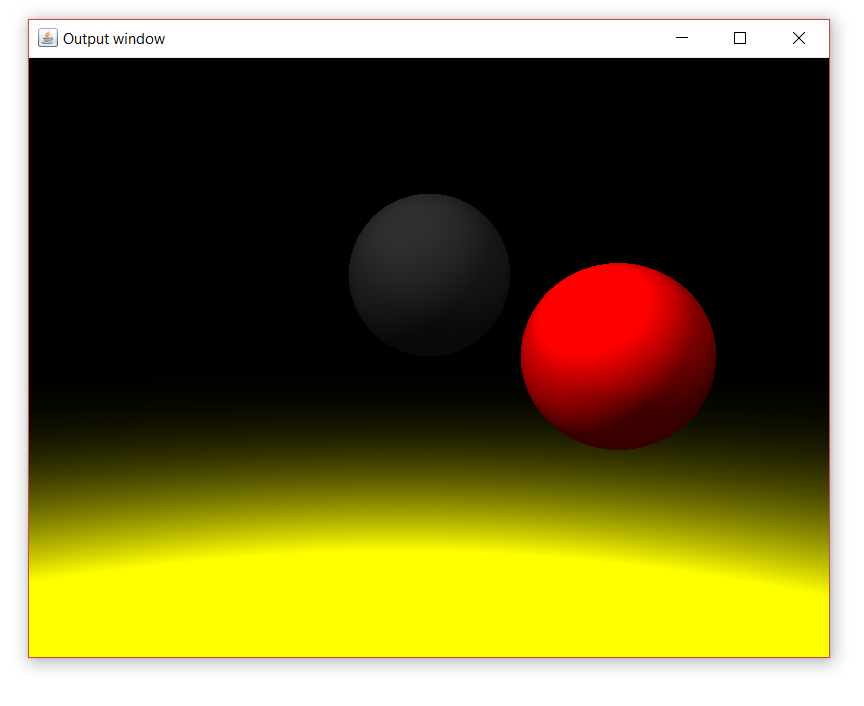
\includegraphics[scale = 0.4]{Figures/10_1.png}
\end{figure}

\subsubsection{Shadows}

Pour créer des ombres, il faut que dans le code qu'on vient d'ajouter, la couleur ne soit modifié pour une lampe que si il n'y a aucun objet entre la lampe et l'endroit ou l'on se trouve.

On modifie alors la condition qui devient 

\begin{lstlisting}
if (cosa>0 && !testShadow(ip, dl)) {
\end{lstlisting}

Et dans la classe \texttt{RayTracing} on implémente la méthode \texttt{testShadow}. A nouveau, le fonctionnement de cette méthode est décrit dans les slides.

\begin{lstlisting}
private boolean testShadow(Vector3 pos, Vector3 dl) {
    for (int i = 0; i < objects.size(); i++) {
        RealObject here = objects.get(i);
        double thit = here.testCollision(pos, dl);
        
        if (thit>0) {
            return true;
        }
    }
    return false;
}
\end{lstlisting}

\begin{figure}[H]
	\caption{\label{10_2} Ombres}
	\centering
	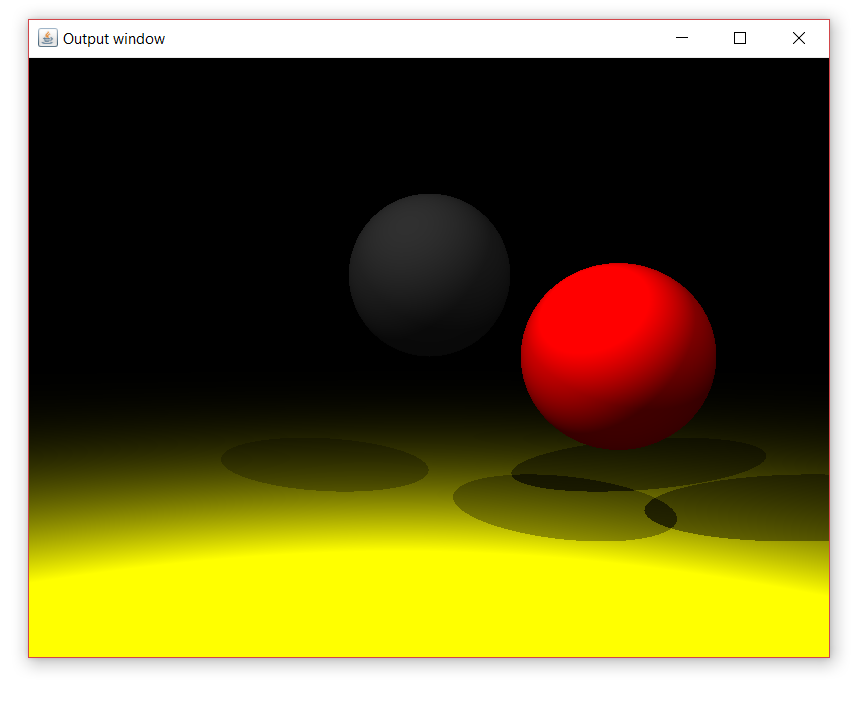
\includegraphics[scale = 0.4]{Figures/10_2.png}
\end{figure}

\subsubsection{Perfect reflection}

Pour implémenter la réflexion, on va devoir modifier les classes représentant les objets pour que leurs constructeurs prennent un paramètre qui sera le coefficient de réflection \texttt{kr}. Voici le code ajouté dans la classe \texttt{PlaneObject} (tout le code n'y est pas, ici se trouve uniquement ce qu'on ajoute pour ajouter le coefficient de réflexion)

\begin{lstlisting}
public class PlaneObject extends RealObject {
    public double kr;
    
    public PlaneObject(Vector3 c, Vector3 n, ColorRGB color, double kr) {
        super(color, kr);
        this.c  = c;
        this.n  = n;
        this.kr = kr;
    }
    
    public PlaneObject(Vector3 c, Vector3 n, ColorRGB color) {
        this(c, n, color, 0.);
    }
}
\end{lstlisting}

On modifie également \texttt{RealObject} pour y ajouter ce coefficient :

\begin{lstlisting}
public final ColorRGB color;
public double kr;

public RealObject(ColorRGB color, double kr) {
    this.color=color;
    this.kr = kr;
}
\end{lstlisting}

On peut alors continuer d'étendre la méthode \texttt{traceRay} pour y ajouter une condition qui, si il y a un coefficient de réflexion, va modifier la couleur en conséquence.

\begin{lstlisting}
// ***** Perfect reflexion *****
if (hittedObject.kr>0) { 
    double dn =2*Vector3.dotProduct(rayDirection, normal);
    Vector3 reflectionDirection = Vector3.subst(rayDirection, Vector3.multiply(normal, dn));
    ColorRGB reflection = traceRay(ip, reflectionDirection);
    
    finalColor.add(ColorRGB.multiply(reflection, hittedObject.kr));
}
\end{lstlisting}

\begin{figure}[H]
	\caption{\label{10_3} Réflexion parfaite}
	\centering
	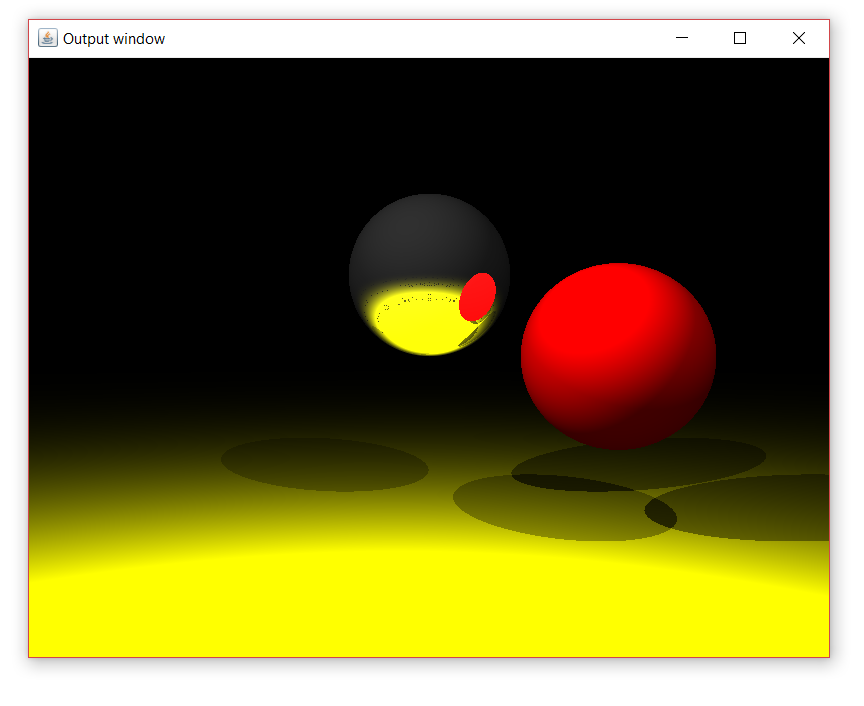
\includegraphics[scale = 0.4]{Figures/10_3.png}
\end{figure}

\subsubsection{Texturing}

Pour créer des surfaces avec des textures, on crée une classe \texttt{TexturizedPlaneObject} qui étends \texttt{PlaneObject}.

\code{raytracing-extended}{TexturizedPlaneObject.java}

On peut alors modifier notre scène dans le constructeur

\begin{lstlisting}
objects.add(new PlaneObject(new Vector3(0, -4, 0), new Vector3(0, 1, 0), yellow));
// devient
objects.add(new TexturizedPlaneObject(new Vector3(0, -4, 0), new Vector3(1, 0, 0), new Vector3(0, 0, 1), green));
\end{lstlisting}

\begin{figure}[H]
	\caption{\label{10_4} Textures}
	\centering
	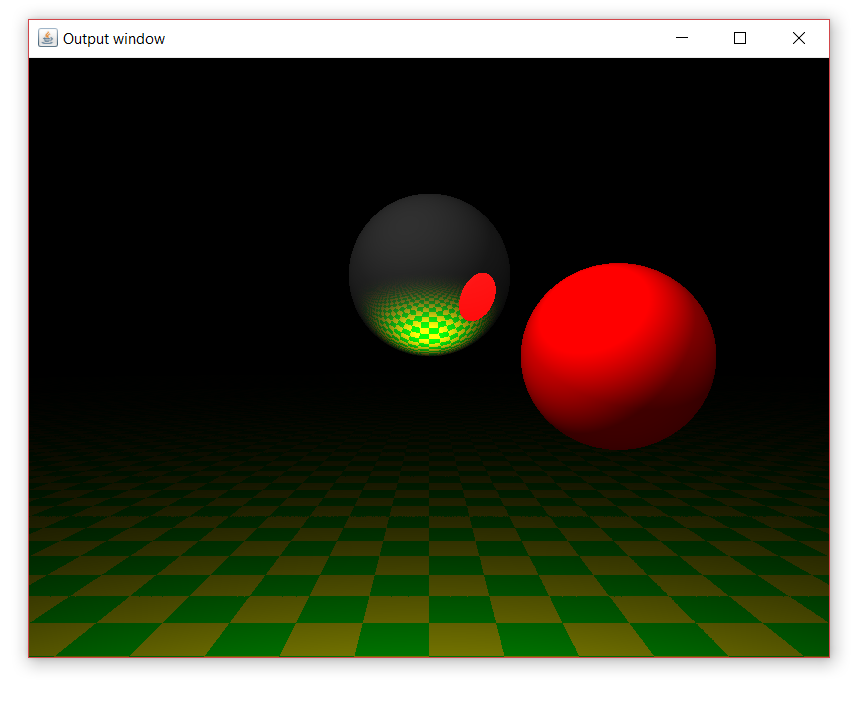
\includegraphics[scale = 0.4]{Figures/10_4.png}
\end{figure}

\subsubsection{Parallelograms}

Pour créer des parallèlogrames, on créer une classe \texttt{ParallelogramObject}. Son fonctionnement est semblable au fonctionnement des plans infinis. La principale différence est la méthode \texttt{testCollision} dont le fonctionnement est développé dans les slides.

\code{raytracing-extended}{ParallelogramObject.java}

On peut alors ajouter un parallèlogramme dans notre scène :

\begin{lstlisting}
objects.add(new ParallelogramObject(new Vector3(-5, -1, 0), new Vector3(0, 0, 5), new Vector3(0, 5, 0), green));
\end{lstlisting}

\begin{figure}[H]
	\caption{\label{10_5} Parallèlogrames}
	\centering
	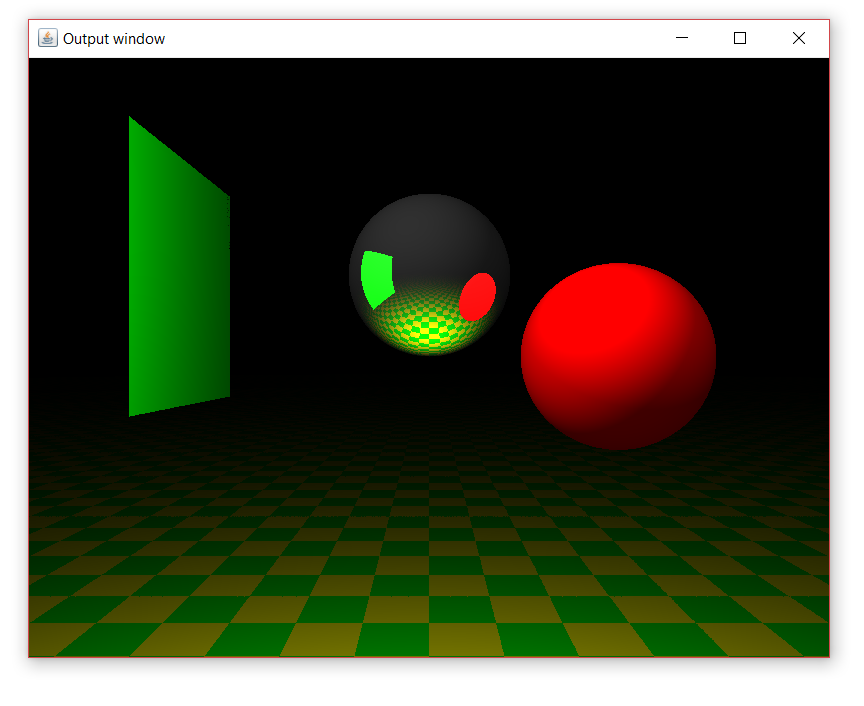
\includegraphics[scale = 0.4]{Figures/10_5.png}
\end{figure}

\begin{figure}[H]
	\caption{\label{10_structure} Diagramme de la structure de raytracing-extended}
	\centering
	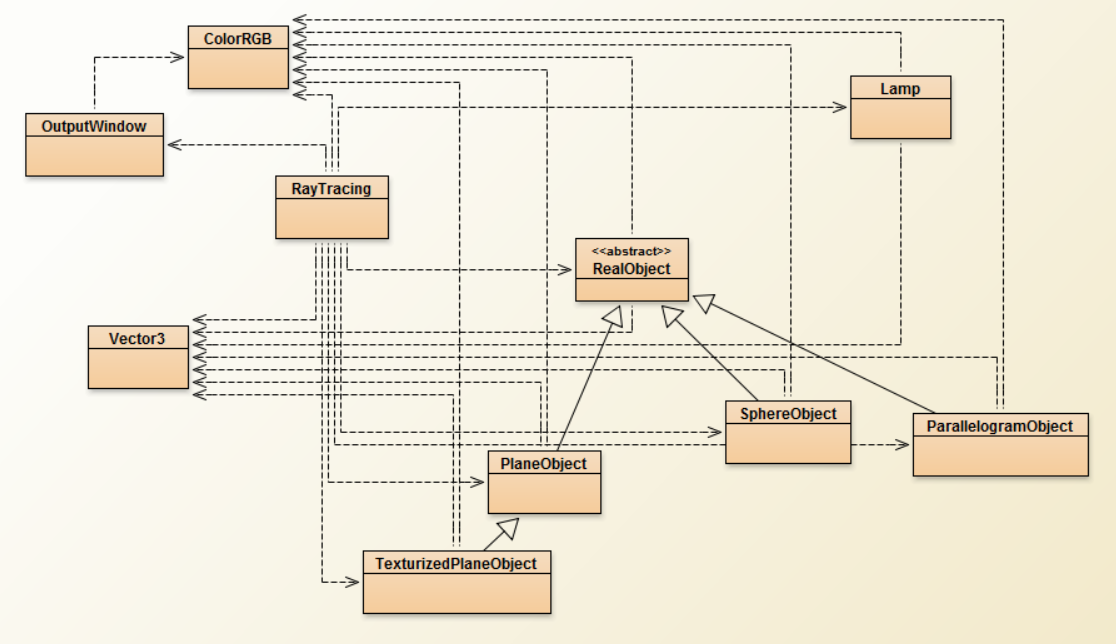
\includegraphics[scale = 0.4]{Figures/10_structure.png}
\end{figure}

\subsection{Question 2}

\subsubsection{Point 1}

Parce que si $cos(\alpha)$ est plus petit que $0$, on est déjà sur que la lampe n'a pas d'influence sur l'objet. Il est donc inutile d'appeler la méthode \texttt{testShadow} qui ferais des calculs inutiles.

\subsubsection{Point 2}

Si l'on place plusieurs objetx avec une réflexion parfaite, on peut avoir des réflexions infinies et donc ne jamais s'arrêter. On peut d'une part arrêter de modifier la couleur si elle est déjà totalement blanche, et d'autre part on peut implémenter un compteur qui limite le nombre de réflexions en chaine à calculer.

\section{Numerical differentiation and solution of nonlinear equations}
\subsection{Question 1}

\begin{equation}
	\begin{aligned}
		p(x) &= \sum_{i=1}^{3}f(x_i)\Phi_i(x\\
		f'(x) &= \sum_{i=1}^{3}f(x_i)\Phi'_i(x)\\
		\Phi_1(x) &= \frac{(x-x_2)(x-x_3)}{(x_1-x_2)(x_1-x_3)} = (x^2 - (x_2+x_3)x+x_2x_3)\frac{1}{(x_1-x_2)(x_1-x_3)}\\
		\Phi_2(x) &= \frac{(x-x_1)(x-x_3)}{(x_2-x_1)(x_2-x_3)}\\
		\Phi_3(x) &= \frac{(x-x_1)(x-x_2)}{(x_3-x_1)(x_3-x_2)}\\
		\Phi_1(x)' &= \frac{2x - (x_2+x_3)}{(x_1-x_2)(x_1-x_3)}\\
		\Phi_2(x)' &= \frac{2x - (x_1+x_3)}{(x_2-x_1)(x_2-x_3)}\\
		\Phi_3(x)' &= \frac{2x - (x_1+x_2)}{(x_3-x_2)(x_3-x_1)}\\
		f'(x) &= f(x_1)\frac{2x - (x_2+x_3)}{(x_1-x_2)(x_1-x_3)} + f(x_2)\frac{2x - (x_1+x_3)}{(x_2-x_1)(x_2-x_3)}+f(x_3)\frac{2x - (x_1+x_2)}{(x_3-x_2)(x_3-x_1)}
	\end{aligned}
\end{equation}

\begin{equation}
	\begin{aligned}
		Erreur &= \frac{f^{(3)}(\xi(x))}{3!}(\prod_{i=1}^{3}(x - x^{(i)}))'\\
		&= \frac{f^{(3)}(\xi(x))}{3!}((x-x_1)(x-x_2)(x-x_3))'\\
		&= \frac{f^{(3)}(\xi(x))}{3!}(x^3-(x_1+x_2+x_3)x^2 + (x_1x_2+(x_1-x_2)x_3)x-x_1x_2x_3)'\\
		&= \frac{f^{(3)}(\xi(x))}{3!}(3x^2 - 2(x_1+x_2+x_3)x + x_1x_2+(x_1+x_2)x_3)\\
	\end{aligned}
\end{equation}

Si l'on remplace $x_1$, $x_2$ et $x_3$ par $x_1 = x-h$, $x_2 = x$ et $x_3 = x + h$, ont obtient :

\begin{equation}
	\begin{aligned}
		f'(x) &= f(x-h)\frac{2x - (x+x+h)}{(x-h-x)(x-h-(x+h))} + f(x)\frac{2x - (x+h+x+h)}{(x-(x-h))(x-(x+h))}\\&\qquad+f(x+h)\frac{2x - (x-h+x)}{(x+h-x)(x+h-(x-h))}\\
		&= f(x-h)\frac{-h}{2h^2} + f(x+h)\frac{h}{2h^2}\\
		&= \frac{f(x+h)-f(x-h)}{2h}
	\end{aligned}
\end{equation}

L'interpolation devient alors identique à la méthode du "two sided centered differencing'' vue au cours.

\subsection{Question 2}

\subsubsection{Point 1}

\begin{equation}
	\begin{aligned}
		T(h) &= \frac{16S(h)-S(2h)}{15} = \frac{2^4S(h)-S(2h)}{2^4-1}\\
		P(h) &= \frac{2^6T(h)-T(2h)}{2^6-1} = \frac{64T(h)-T(2h)}{63}
	\end{aligned}
\end{equation}

\subsubsection{Point 2}

\begin{equation}
	\begin{aligned}
		\begin{cases} 
			R_0(h) = D(h)\\
			R_i(h) = \frac{2^{2i}R_{(i-1)}(h) - R_{(i-1)}(2h)}{2^{2i}-1}
		\end{cases}
	\end{aligned}
\end{equation}

\subsubsection{Point 3}

\begin{equation}
	\begin{aligned}
		\begin{cases} 
			R_0(h) = D(h)\\
			R_i(h) = \frac{2^{2i}R_{(i-1)}(h) - R_{(i-1)}(\alpha h)}{2^{2i}-1}
		\end{cases}
	\end{aligned}
\end{equation}

// A CONFIRMER

\subsection{Question 3}

\subsubsection{Point 1}

\paragraph{$f$ differentiable but $f'$ is expensive to evaluate}

Si $f$ est diiférentiable mais chèr à évaluer, on peut utiliser la 'secant method'. Avec cette méthode on va approximer en ré-utilisant ce qu'on a déjà calculé lors des itérations précédentes.

\begin{equation}
	\begin{aligned}
		f'(x_k) &\approx \frac{f(x_k) - f(x_{k-1})}{x_k-x_{k-1}}\\
		x_{k+1} &= x_k - \frac{f(x_k)(x_k-x_{k-1})}{f(x_k)-f(x_{k-1})}
	\end{aligned}
\end{equation}

\paragraph{$f$ is continuous but not differentiable}

Si $f$ est continue mais pas différentiable, on peut utiliser le 'bisection algorithm'.

\begin{equation}
	\begin{aligned}
		f(a) < u < f(b)\quad &\text{ou} \quad f(a) > u > f(b)\\
		&\exists z \in [a, b] \text{ tq } f(z) = u
	\end{aligned}
\end{equation}

\subsubsection{Point 2}

// TO DO

\subsubsection{Point 3}

\begin{equation}
	\begin{aligned}
		Cost(f(x)) &= t\\
		Cost(f'(x)) &= \frac{t}{2}
	\end{aligned}
\end{equation}

On va calculer pour chaque méthode combien de fois on doit calculer $f(x)$ et $f'(x)$ lors d'une itération pour pouvoir estimer le cout de chaque méthode. La méthode qui aura le cout d'une itération le plus bas sera préférée.

\paragraph{Newton-Raphson}Avec la méthode de Newton-Raphson, lors d'une itération on calcule une fois $f(x)$ et une fois $f'(x)$

\begin{equation}
	\begin{aligned}
		Cost(Newton-Raphson) &= 1 \cdot Cost(f(x)) + 1 \cdot Cost(f'(x))\\
		&= t + \frac{t}{2} = \frac{3t}{2}
	\end{aligned}
\end{equation}

\paragraph{Secant method}Avec la méthode sécante, lors d'une itération on calcule trois fois $f(x)$ et on ne calcule jamais $f'(x)$.

\begin{equation}
	\begin{aligned}
		Cost(Secant) &= 3 \cdot Cost(f(x)) + 0 \cdot Cost(f'(x))\\
		&= 3t
	\end{aligned}
\end{equation}

Pour les couts donnés, la méthode sécante coute deux fois plus que la méthode de Newton-Raphson, qui sera donc préférée dans ce cas.

\subsection{Question 4}

\subsubsection{Point 1}

\code{littleclasses}{NewtonRaphson.java}

Quelques commentaires sur le code ;

\begin{itemize}
\item La méthode \texttt{getIteration} calcule une itération
\item \texttt{process} calcule la racine pour un $x_0$ donné et une erreur acceptable
\item En plottant le fichier créé par la méthode \texttt{saveData} on peut voir le nombre d'itérations nécessaire en fonction du $x_0$
\end{itemize}

\subsubsection{Point 2}

Avec la méthode \texttt{main}, on va calculer la racine avec la méthode de Newton-Raphson pour 100 points répartis uniformément entre $-10$ et $10$. On peut voir sur le graphique le nombre d'itérations nécessaires en fonction du $x_0$ choisi.

\begin{figure}[H]
	\caption{\label{11_newton_raphson} Nombre d'itérations en fonction du $x_0$ choisi}
	\centering
	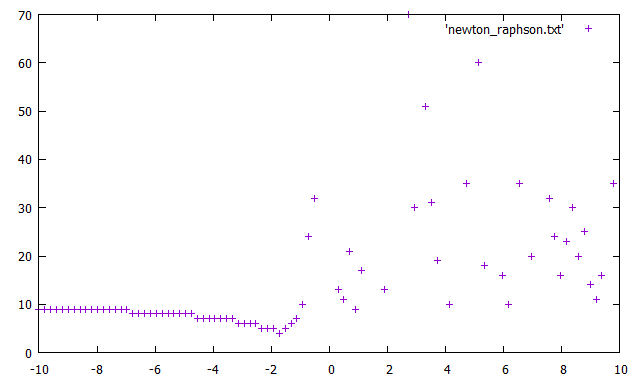
\includegraphics[scale = 0.6]{Figures/11_newton_raphson.png}
\end{figure}

A l'aide de la méthode \texttt{displayNoConvergence} on peut récupérer les $x_0$ pour lesquels Newton-Cotes ne converge pas. Voici la liste des points qui après 200 itérations n'ont pas trouvé de solution :

\begin{table}[H]
\centering
\begin{tabular}{|c|}
\hline
-0.30303030303030276\\
-0.10101010101010033\\
0.10101010101010033\\
1.3131313131313131\\
1.5151515151515156\\
1.7171717171717162\\
2.121212121212121\\
2.3232323232323235\\
2.525252525252524\\
3.1313131313131315\\
3.9393939393939394\\
4.3434343434343425\\
4.545454545454545\\
4.94949494949495\\
5.555555555555555\\
5.757575757575758\\
6.363636363636363\\
6.767676767676768\\
7.171717171717173\\
7.373737373737374\\
9.595959595959595\\
10.0\\
\hline
\end{tabular}
\end{table}
\subsubsection{Point 3}

On peut déduire du graphique qu'au plus $x_0$ est loin de la racine, au plus le nombre d'itérations nécessaires est élevé.

\subsection{Question 5}

\subsubsection{Point 1}

// TO DO

\subsubsection{Point 2}

// TO DO

\section{Initial value problems}
\subsection{Question 1}

\subsubsection{Point 1}

\begin{equation}
	\begin{aligned}
		f(x) &= \frac{1}{C - x} + x\\
		f(2) &= 1\\
		1 &= \frac{1}{C - 2} + 2\\
		C &= 1
	\end{aligned}
\end{equation}

Pour que l'IVP soit stable, il faut que $\frac{\delta F}{\delta f}|_{(x_i, \zeta_i)}<0$

\begin{equation}
	\begin{aligned}
		\frac{\delta F}{\delta f}|_{(x_i, \zeta_i)} &= \frac{\delta}{\delta f} (1+(x-f(x))^2)\\
		&= (2f(x)-2x)|_{(x_i, \zeta_i)}\\
		(2f(x)-2x) &<0\\
		f(x)-x &< 0\\
		\frac{1}{1-x}+x-x&<0
	\end{aligned}
\end{equation}

Si on vérifie cette dernière inéquation pour tous les $x$ d'intéret (à savoir $x \geq 2$), on constate qu'elle est toujours vérifiée. L'IVP est donc stable pour les valeurs d'intérêt.

\subsubsection{Point 2}

\begin{equation}
	\begin{aligned}
		f_2 &= 1\\
		f_{i+1} &= h(1 + (x_i - f_i)^2)+f_i\\
	\end{aligned}
\end{equation}

Pour que les itérations soient stable, il faut que $h < \frac{-2}{\frac{\delta F}{\delta f}|_{(x_i, \zeta_i)}}$

\begin{equation}
	\begin{aligned}
		h &< \frac{-2}{\frac{\delta F}{\delta f}|_{(x_i, \zeta_i)}}\\
		&< \frac{-2}{2f(x)-2x}\\
		&< \frac{-1}{f(x)-x}\\
		&< \frac{-1}{\frac{1}{1-x}+x-x}\\
		&< x-1
	\end{aligned}
\end{equation}

Il faut donc choisir un $h$ plus petit que $1$ pour que les itérations soient stable.

\subsubsection{Point 3}

\code{littleclasses}{ForwardEuler.java}

Pour adapter le code à une autre fonction, il faut modifier les variables dans la méthode \texttt{main} ainsi que la méthode \texttt{F}. Il est également possible de mettre la fonction exacte dans la méthode \texttt{exactFunction} et de mettre alors le booléen \texttt{compareWithExactFunction} à \texttt{true}. Dans ce cas, le tableau renvoyé par la méthode \texttt{process} contiendra une troisième colonne avec les évaluations pour ces $x$ de la fonction exacte. On peut alors créer un graphe pour comparer les résultats obtenus par Forward Euler et les valeurs exactes avec gnuplot par exemple via la commande suivante :

\begin{lstlisting}
plot 'forward_euler.txt' using 1:2 with lines title 'Forward Euler', '' using 1:3 with lines title 'Exact function'
\end{lstlisting}

\begin{figure}[H]
	\caption{\label{12_forward_1} Forward Euler avec $h=0.25$}
	\centering
	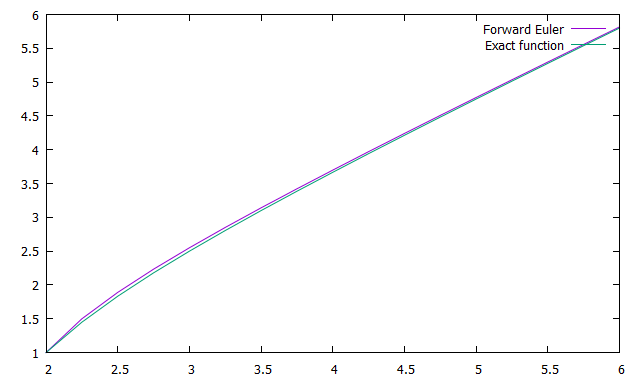
\includegraphics[scale = 0.6]{Figures/12_forward_1.png}
\end{figure}


\subsection{Question 2}

\begin{equation}
	\begin{aligned}
	\begin{cases}
	f'(x) = x + \sqrt{f(x)}\\
	f(1) = 2
	\end{cases}
	\end{aligned}
\end{equation}

Pour l'implémentation de Forward Euler, il nous suffit d'adapter l'implémentation de la question précédente en modifiant les variables de la valeur initiale et la méthode \texttt{F}. Pour le Classical Runge-Kutta on peut très simplement l'implémenter en se basant sur la structure de notre implémentation pour Forward Euler.

\code{littleclasses}{RK4.java}

\subsubsection{Point 1}

// TO DO

\subsubsection{Point 2}

Pour calculer le plus grand $h$ qui nous permette d'obtenir une solution exacte arrondie à 4 décimales, on peut utiliser une boucle qui commence avec un grand $h$ et le réduit tant que la différence entre la solution obtenue et le solution exacte est trop grande. Cette technique a été implémentée dans la méthode \texttt{calculate\_biggest\_h} et on peut ainsi déterminer que le plus grand $h$ qui nous permets d'obtenir une solution exacte est $0.2$.

\subsubsection{Point 3}

// TO DO

\subsection{Question 3}

\begin{equation}
	\begin{aligned}
	\begin{cases}
	f'(x) = sin(f(x))\\
	f(0) = 1
	\end{cases}
	\end{aligned}
\end{equation}

\begin{equation}
	\begin{aligned}
		f(x_{i+1}) \approx f_{i+1} &= hF(x_{i+1}, f_{i+1}) + f_i\\
		&= h\cdot sin(f_{i+1}) + f_i
	\end{aligned}
\end{equation}
// TO DO

\subsection{Question 4}

\subsubsection{Point 1}

// TO DO

\subsubsection{Point 2}

// TO DO

\section{Initial value problems (part 2)}
\subsection{Question 1}



// TO DO


\end{document}
